\chapter{Results}
\label{chap:4_results}

This chapter describes the different experiments and benchmarks applied to the proposed system and its subsystems. These tests have the purpose of taking design or implementation decisions, selecting the best choices to improve performance, accuracy and robustness of the final system and subsystems. For this purpose, several video sequences were recorded with the ASUS Xtion inside ROSBag files. This way, the same video can be used to assess the performance of different configurations, ensuring that the results will not be affected by external variability due to different environmental conditions on the test data.\\

The majority of the tests described below for the neural pipeline measure the IoU score (\autoref{fig:2_iou}), which determines the overlapping quality between two bounding boxes. Thus, it is required to label the video sequences, specifying on each frame the location of the ground truth labels for every video. For this purpose, the tool LabelMe \cite{labelme} was used to provide the labels to the video, creating a JSON file for each frame of the video sequence. A screenshot of this tool is shown on \autoref{fig:4_labelme}.\\

The source code of the experiments conducted below can be found in a separate \texttt{experiments} branch of the source repository on GitHub\footnote{\url{https://github.com/RoboticsLabURJC/2017-tfg-nacho_condes/tree/experiments}}, hosting both the testing and plotting source files, as well as the CSV files containing the data plotted in the figures below.


\begin{figure}[h]
	\centering
	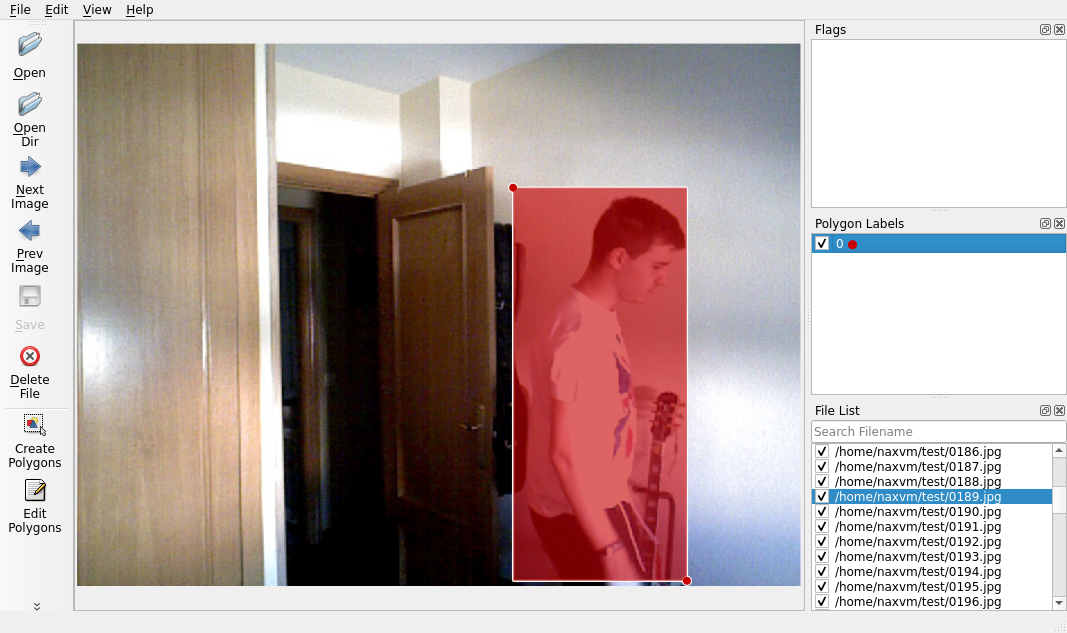
\includegraphics[width=0.8\linewidth]{labelme}
	\caption{Interface of the LabelMe annotation tool \cite{labelme}.}
	\label{fig:4_labelme}
\end{figure}


\section{Person detection experiments}
\label{sec:4_test1}
This experiment compares the two detection architectures implemented on this system: YOLO \cite{yolov3} and SSD\cite{ssd}.

In the case of YOLO, the implemented architecture is YOLOv3, in its \textit{tiny} version. This is due to the memory constraints of the Jetson board where the models are loaded. The available memory (8 GB) has to be shared among TensorFlow and the rest of processes, causing the more memory-intensive models to fail on loading. The YOLOv3 full model demands too much memory, making impossible to use it properly on the Jetson TX2 board. Thus, the chosen architecture is a lighter one, publicly available on the YOLO website\footnote{\url{https://pjreddie.com/darknet/yolo/}}: the Tiny YOLOv3 model.

On the other hand, as it was explained in Chapter \ref{chap:2_sota}, on a real-time application the most convenient variant of the SSD-based detectors is the one that uses a MobileNet \cite{mobilenet} as a feature extraction network. The TensorFlow Model Zoo \cite{model_zoo} offers several pre-trained models implementing this network, along which a selection has been carried out (as it will be described in other tests). The chosen model integrates a MobileNetv1 whose weights have been quantized \cite{ssd_quantization} in order to reduce the computational cost without reducing the accuracy.\\


In order to quantify the different accuracy vs. inference time tradeoffs that these architectures offer, a specific test has been designed. A specific video sequence of 721 frames long has been recorded, containing a person wandering across the field of view of the camera. Several extracted frames from this sequence can be observed on \autoref{fig:4_test1_frames}. For every frame of the sequence, the persons are detected using YOLO and SSD respectively, and the IoU and the inference time have been measured, as it can be seen on \autoref{fig:4_test1_results}. Some gaps can be noticed on the detections, corresponding to the frames where the person was out of the sight of the camera.

\begin{figure}[h]
	\centering
	\begin{subfigure}[b]{0.3\linewidth}
		\centering
		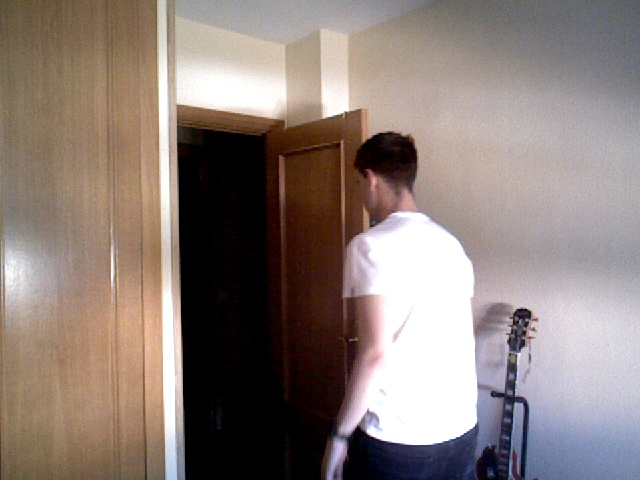
\includegraphics[width=0.95\linewidth]{test1_1}
		\caption{Frame 322.}
	\end{subfigure}
	\begin{subfigure}[b]{0.3\linewidth}
		\centering
		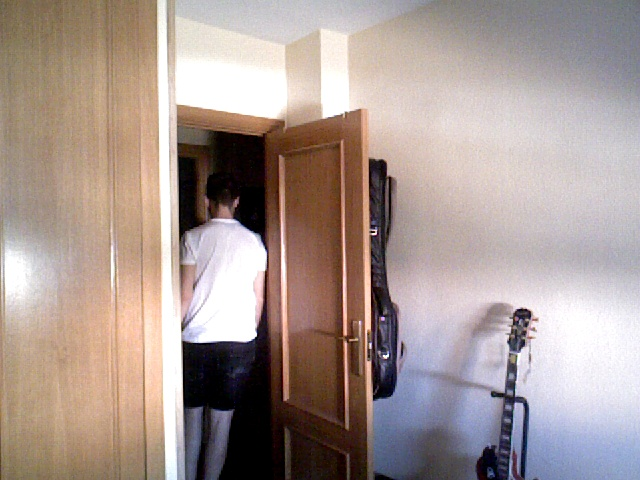
\includegraphics[width=0.95\linewidth]{test1_2}
		\caption{Frame 479.}
	\end{subfigure}
	\begin{subfigure}[b]{0.3\linewidth}
		\centering
		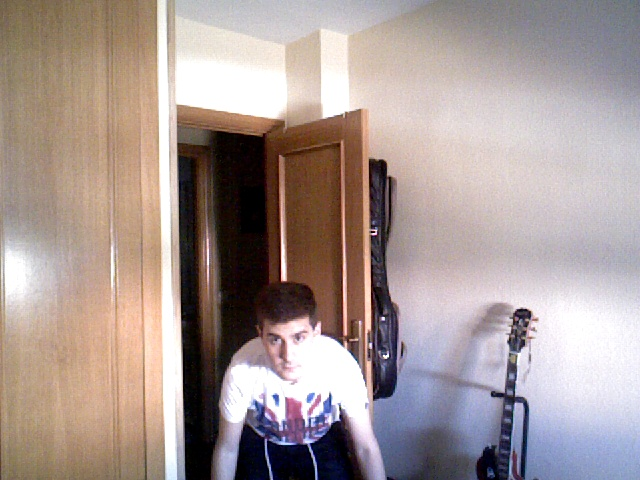
\includegraphics[width=0.95\linewidth]{test1_3}
		\caption{Frame 648.}
	\end{subfigure}
	\caption{3 frames from the test video sequence.}
	\label{fig:4_test1_frames}
\end{figure}



\begin{figure}[h]
	\centering
	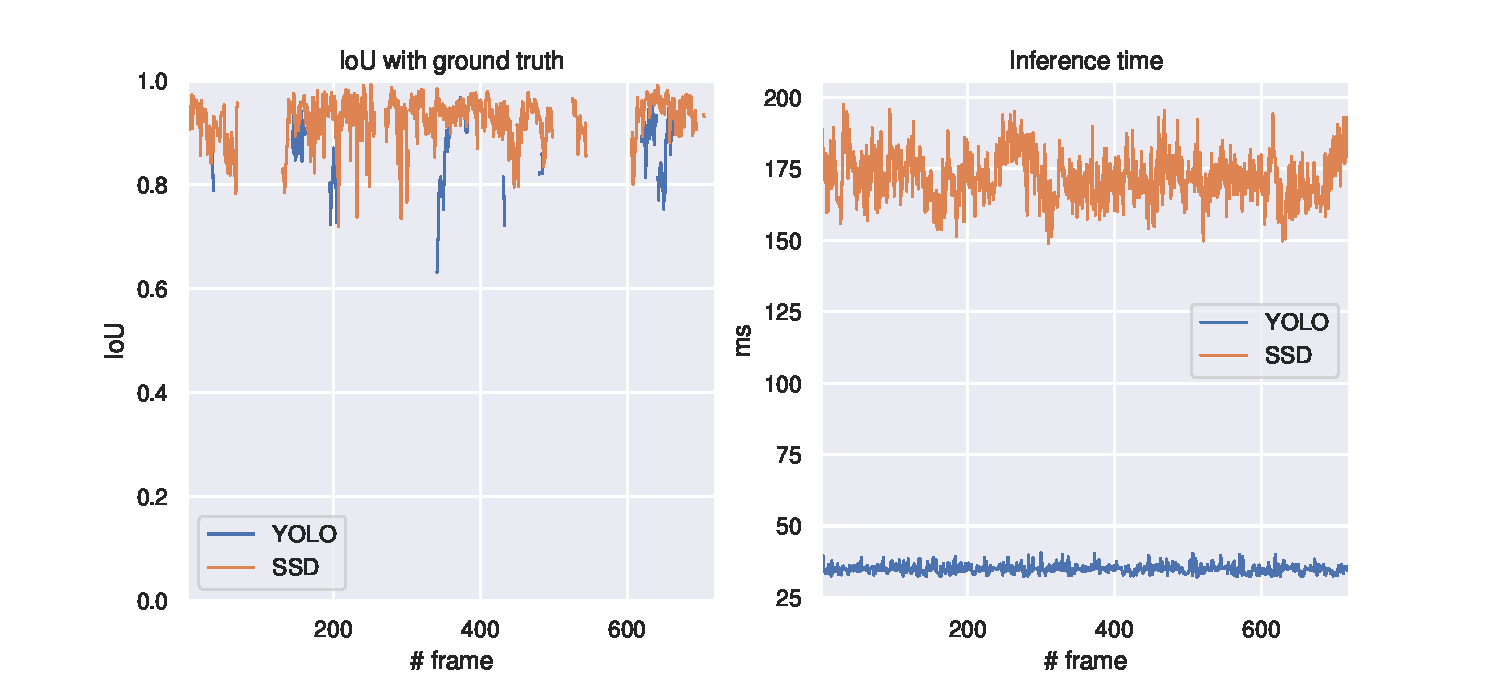
\includegraphics[width=0.95\linewidth]{test1}
	\caption{Results of the person detection test: IoU score with ground truth (left) and inference time per frame (right). A discontinuity represents absence of detections.}
	\label{fig:4_test1_results}
\end{figure}

\begin{table}[h]
	\begin{tabular}{|l|c|c|}
		\hline
		& \textbf{YOLO}             & \textbf{SSD}              \\ \hline
		\textbf{IoU}            & 0.858 $\pm$  0.068 & 0.926 $\pm$  0.044 \\ \hline
		\textbf{Inf. time (ms)} & 35.003 $\pm$ 1.503 & 172.237 $\pm$ 8.791 \\ \hline
		\textbf{Frames with detection} & 123 (17.06\%) & 533 (73.93\%) \\ \hline
	\end{tabular}
	\caption{Numeric summary (average $\pm$ standard deviation) for the person detection experiment.}
	\label{tab:4_test1}
\end{table}

The two outstanding object detection architectures have been compared, using both to extract inferences on the same video sequence. The results can be visualized on \autoref{fig:4_test1_results} and summarized on \autoref{tab:4_test1}. The YOLO-based detector offers a slightly minor IoU than the SSD-based one (around 0.858 and 0.926 respectively), while taking 5 times less time to make inferences (35 ms vs. 172 ms). On these terms, the YOLO-based detector seems much more efficient. However, \autoref{tab:4_test1} shows as well a very unstable detection in the YOLO case, being able to detect the person only in 17\% of the frames, whereas SSD detects the person successfully in 74\% of the cases. In fact, as there are several frames where the person is not seen, SSD is successful practically in all the cases.\\
This shows that the YOLO detector is too dependent on pose and lighting conditions for the detections to be successful. On the other hand, the SSD detector yields steady predictions, only cutting on the periods where the person was truly out of the field of view. Hence, this system is much more robust for our application scenario.\\

One fundamental requirement of the system is the real-time behavior, which makes inference time an important factor to be taken into account. However, as the system includes the described optical tracker, the YOLO detector can be discarded in favor of the SSD-based one, given that the YOLO version has a much lower detection rate\footnote{As it was described before, the implemented version of the YOLO detector is \textit{Tiny YOLOv3}, due to the memory requirements for deploying the full YOLOv3 model, which are higher than what the Jetson TX2 can handle. Thus, it is probable to expect a better performance on the full model in a different computer capable of handling it.} and this can not be palliated by the motion tracker.\\



\section{Face detection experiments}
\label{sec:4_test2}

One of the improvements of the proposed system over the previous work \cite{tfg} is the utilization of a fully neural detection pipeline, as it was described on Chapter \ref{chap:3_materials_methods}. This requires the replacement of the face detection Haar cascade classifier explained on Chapter \ref{chap:2_sota} by a neural alternative: \textit{faced}.\\

 This experiment is devoted to compare the performance of both face detection systems. Its design is similar to the previous experiment, using the same video sequence (\autoref{fig:4_test1_frames}) with the ground truth faces labeled using LabelMe. For each frame in the sequence, the faces are extracted using each one of the described methods, and the IoU score is computed with the ground truth face bounding box. The result can be visualized in \autoref{fig:4_test2_results}.

\begin{figure}[h]
	\centering
	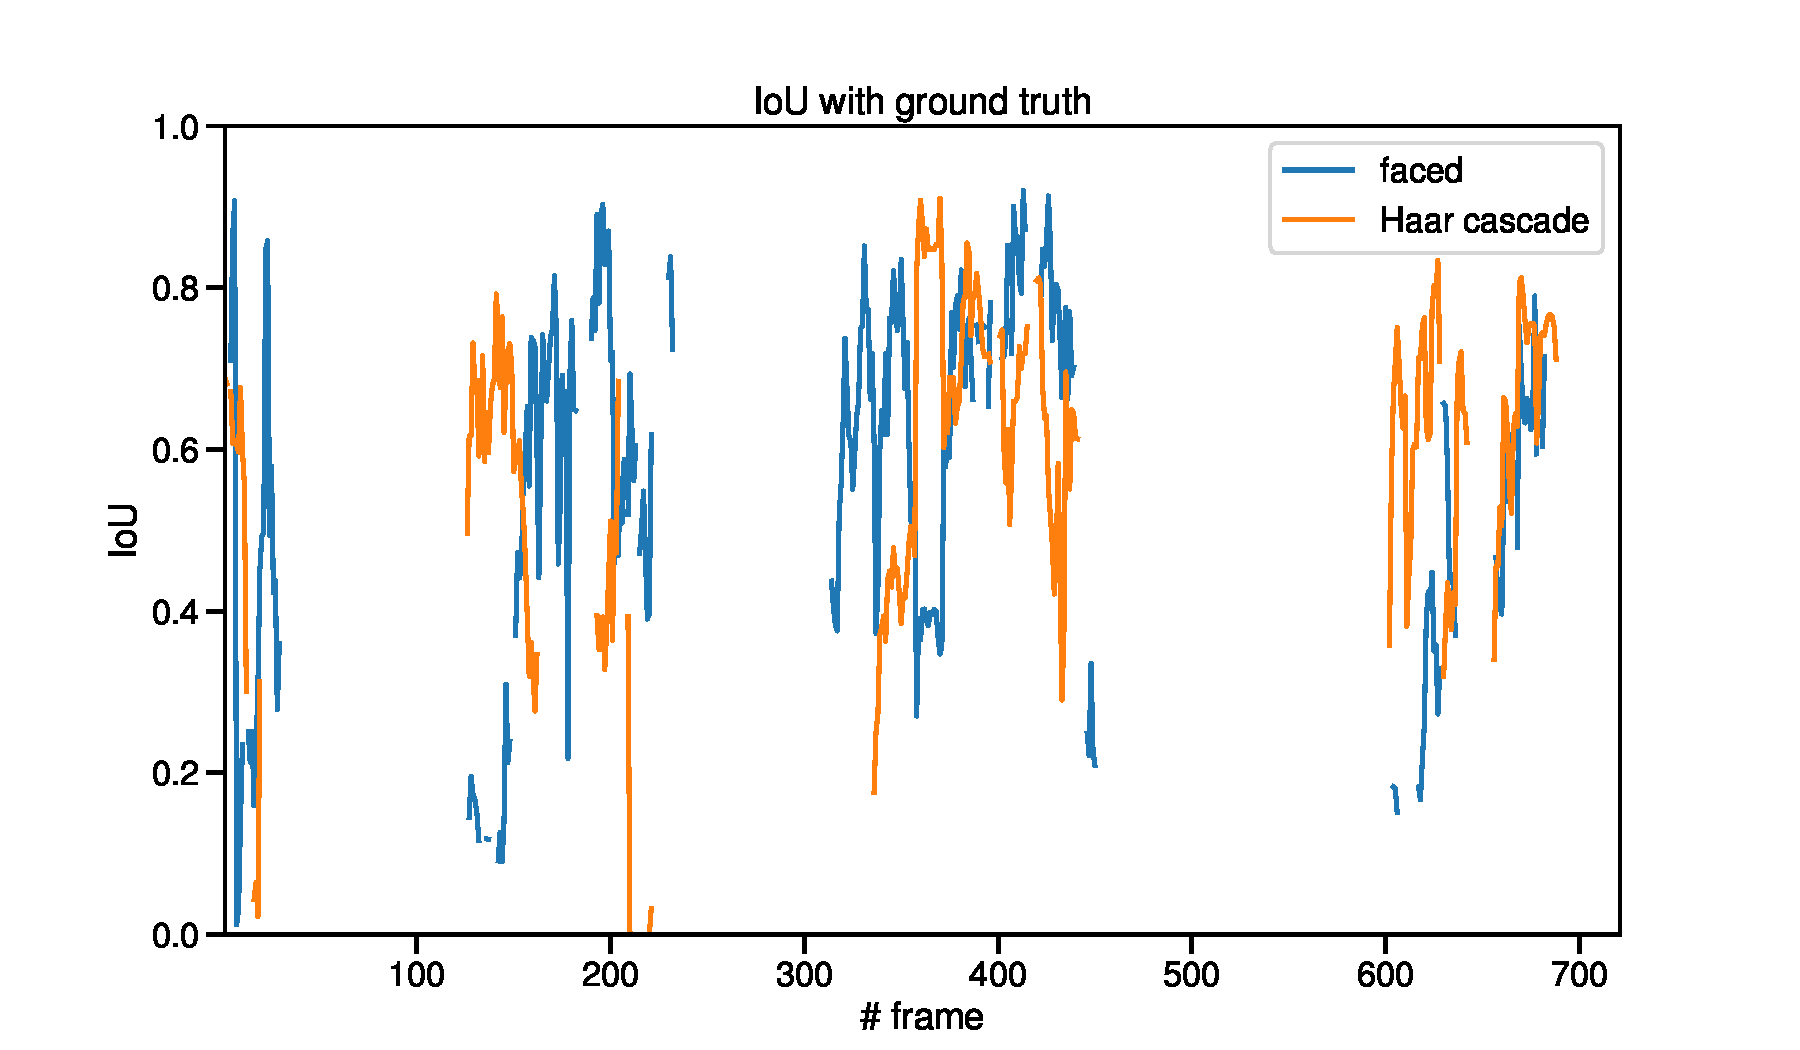
\includegraphics[width=0.6\linewidth]{test2}
	\caption{IoU score with the ground truth for each one of the face detection systems.}
	\label{fig:4_test2_results}
\end{figure}

\begin{table}[h]
	\begin{tabular}{|l|c|c|}
		\hline
		& \textbf{haar}             & \textbf{faced}              \\ \hline
		\textbf{IoU}            & 0.579 $\pm$  0.202 & 0.559 $\pm$  0.221 \\ \hline
		\textbf{Frames with detection} & 248 (34.40\%) & 266 (36.89\%) \\ \hline
	\end{tabular}
	\caption{Numeric summary (average $\pm$ standard deviation) for the face detection experiment.}
	\label{tab:4_test2}
\end{table}


\autoref{fig:4_test2_results} and \autoref{tab:4_test2} show the detection scores for the two mentioned systems on the same video sequence. It can be seen that both yield similar IoU scores and drop at the same time when the person turns their back to the camera. However, the \texttt{faced} implementation (which uses deep learning to predict the face positions) is capable of keeping a non-zero IoU at several instants where the Haar performance drops to zero.  This is due to pose variances of the person, as the main drawback of the Haar cascade classifier is that it is only capable of detecting frontal faces, dropping the performance whenever the person turns the face towards a side. This effect is observable in \autoref{tab:4_test2}, since both methods yield similar IoU on average, but the deep-learning approach, \texttt{faced}, detects a face in 36.89\% of the frames, whereas the Haar cascade slightly drops the detection rate to 34.40\%.\\

Hence, this test validates the improvement of the face detection performance when using a specific neural network trained for that purpose.




\section{Face recognition experiments}

\label{sec:4_test4}
The last component of the neural pipeline is a \textit{face recognition} neural network, devoted to confirm the identity of the reference person. This is useful for discerning whether that person has to be followed even if they turns back later, as their position is tracked with the described means. This subsystem is based on a FaceNet \cite{facenet} network, which projects a face into a 128-dimensional space. These projections are used by the proposed system, as their euclidean distance to the projection of a reference face is used to determine if the input face belongs to the reference person.\\

This experiment is designed to assess the quality of the projection system, which should yield far points for a different face and near points for a matching face. For this proposal, a video sequence was recorded containing two persons wandering in front of the robot. The faces of each frame are labeled, separating the faces of the two persons in two different classes. A caption of the video with the labels can be seen on \autoref{fig:4_test4_labelme}. \autoref{fig:4_test4_frames} shows several frames from the sequence as well, where some occlusions on the faces can be observed. 

\begin{figure}[h]
	\centering
	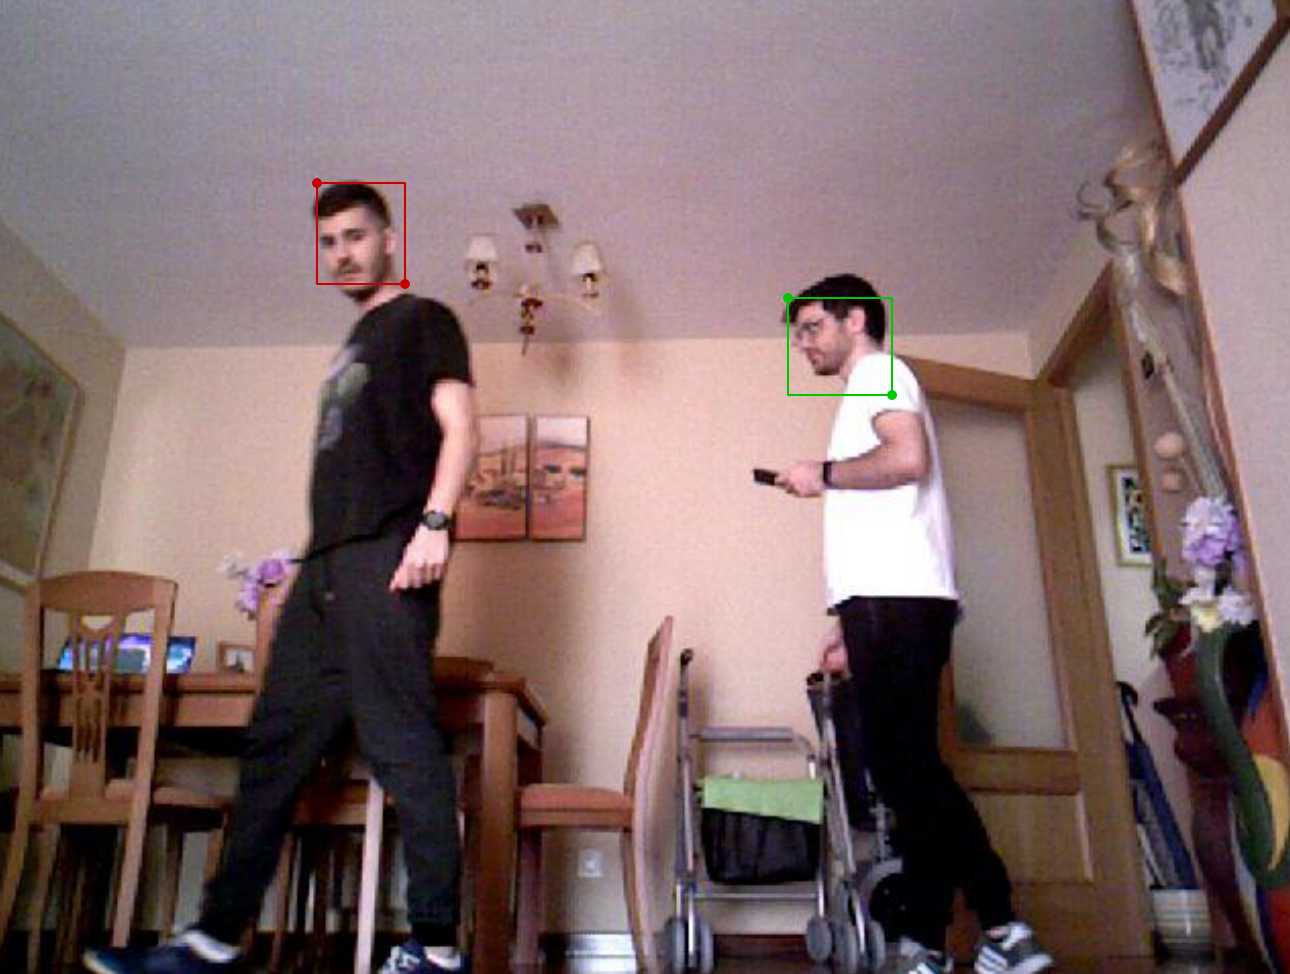
\includegraphics[width=0.6\linewidth]{test4_labelme}
	\caption{A frame of the test sequence showing the labels on the faces.}
	\label{fig:4_test4_labelme}
\end{figure}



\begin{figure}[h]
	\centering
	\begin{subfigure}[b]{0.3\linewidth}
		\centering
		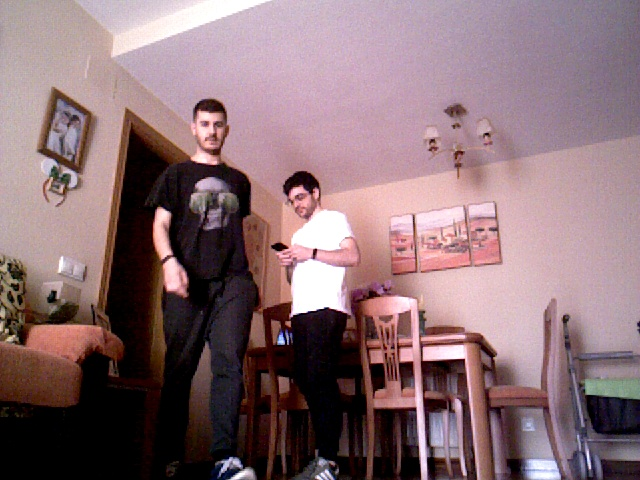
\includegraphics[width=0.95\linewidth]{test4_1}
		\caption{Frame 74.}
	\end{subfigure}
	\begin{subfigure}[b]{0.3\linewidth}
		\centering
		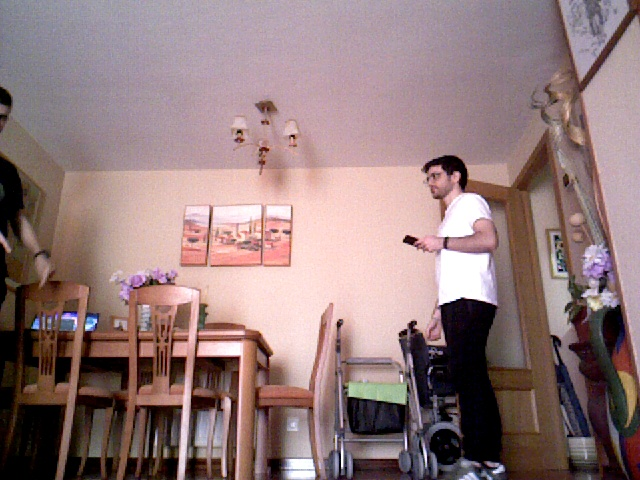
\includegraphics[width=0.95\linewidth]{test4_2}
		\caption{Frame 735.}
	\end{subfigure}
	\begin{subfigure}[b]{0.3\linewidth}
		\centering
		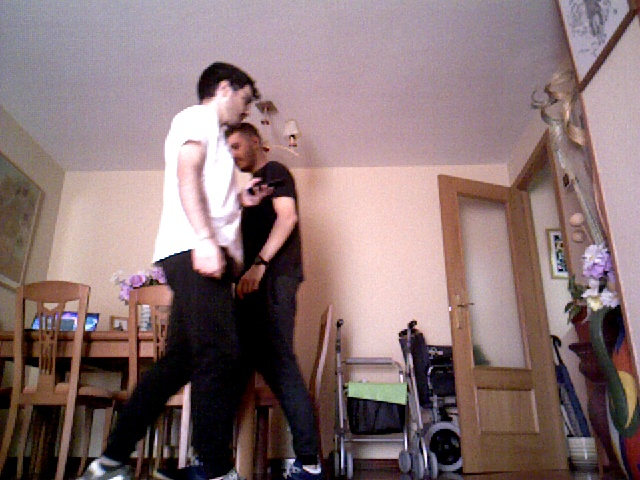
\includegraphics[width=0.95\linewidth]{test4_3}
		\caption{Frame 1136.}
	\end{subfigure}
	\caption{3 frames from the test video sequence.}
	\label{fig:4_test4_frames}
\end{figure}


For computing the distance, the reference face was set using the image on \autoref{fig:4_test4_refface}, and the distance to the reference face of each one of the faces in the video was stored. The result can be observed on \autoref{fig:4_test4_result}.


\begin{figure}[h]
	\centering
	\begin{subfigure}[b]{0.25\linewidth}
		\centering
		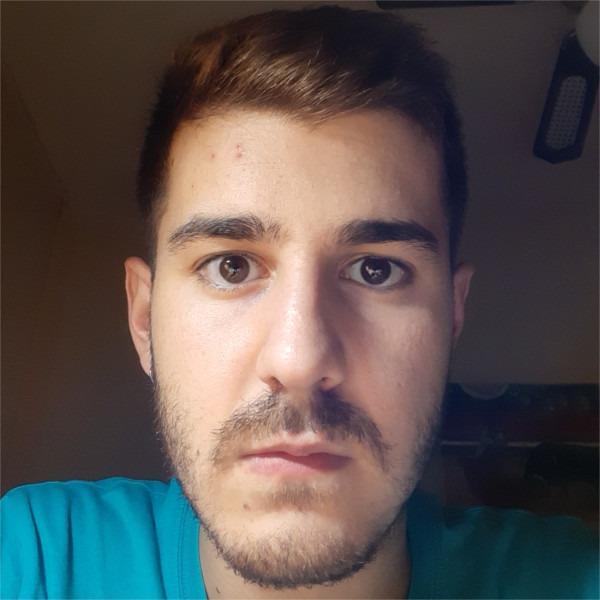
\includegraphics[width=0.95\linewidth]{test4_refface}
		\caption{Image of the reference face.}
		\label{fig:4_test4_refface}
	\end{subfigure}
	\hfill
	\begin{subfigure}[b]{0.7\linewidth}
		\centering
		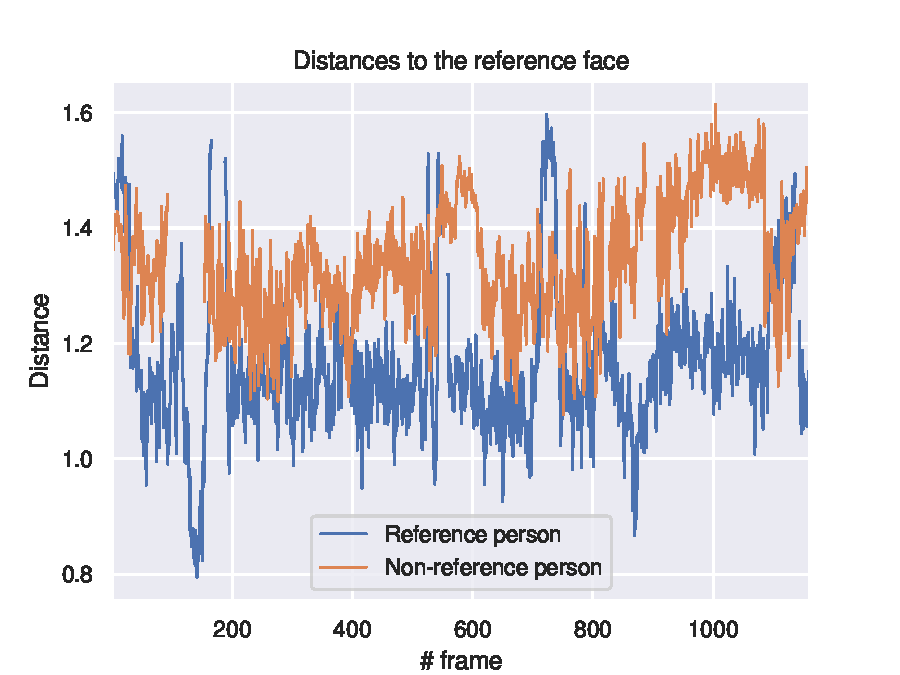
\includegraphics[width=0.95\linewidth]{test4}
		\caption{Resulting distance for the two faces present in the video.}
		\label{fig:4_test4_result}
	\end{subfigure}
	\caption{Results of the face recognition experiment. (a): reference face used for the test. (b): distance of each face to the reference projection of (a).}
	\label{fig:4_test4}
\end{figure}


\begin{table}[h]
	\begin{tabular}{|l|c|c|}
		\hline
		& \textbf{Ref. person} & \textbf{Non-ref. person} \\ \hline
		\textbf{IoU}           & 1.160 $\pm$  0.128 & 1.344 $\pm$  0.102 \\ \hline
	\end{tabular}
	\caption{Numeric summary (average $\pm$ standard deviation) for the face recognition experiment.}
	\label{tab:4_test4}
\end{table}


The results obtained on \autoref{fig:4_test4} and \autoref{tab:4_test4} allow to extract two conclusions about the quality of the projections of the faces:

\begin{itemize}
	\item The encodings of the reference person (the person with the same face than the reference one) have an overall remarkable stability. In average, the obtained projections for every frame are located at an approximate distance of $1.16$ (threshold chosen for accepting a person as the reference one). Exceptional rises in the distance can be found as well, but they are due to changes in the pose of the face and occlusions, that reduce the quality of the projection.\\
	\item The encodings of a person different than the reference one have an overall higher distance from the reference face. This is convenient for avoiding false positives while determining that a face is the reference one.
\end{itemize} 

This allows to conclude a correct performance of the triplet loss (\autoref{fig:2_facenet_triplet_loss}) on which a FaceNet is trained \cite{facenet}. This yields an efficient separation between the encodings of different persons, as well as close encodings for faces belonging to the same person, making this system a robust approach to perform person recognition tasks, since the distance of a projection to the reference face has to be below the threshold for being labeled as the reference face.\\



\section{TensorRT experiments}

\subsection{Performance tuning the optimization parameters}
\label{sec:4_grid_trt}

In Section \ref{sec:3_design}, the TensorRT engine was introduced. This engine is used to optimize, using a binding component between TensorFlow network graphs and TensorRT itself, the implementation of a neural network on a compatible NVIDIA GPU. There are several tunable parameters for customizing the implementation, and the most relevant ones were described in Section \ref{sec:3_design} as well. As varying these parameters changes the model size and the inference time, an experiment has been conducted in order to test the inference time of each model. The optimization script performs a grid search between a set of values for each parameter (MSS, MCE and precision mode, as described on Section \ref{sec:3_design}), and tests the performance on a specific ROSBag sequence, storing the detections and the inference times on a YAML file, besides the optimized graph to be loaded without requiring to perform the optimization again.\\

The inference times for the fastest SSD-based model and the Tiny YOLOv3 implementations are shown below in \autoref{tab:4_ssd_trt_results} and \autoref{tab:4_yolo_trt_results}. The impact of this optimization on the precision is studied on Subsection \ref{sec:4_test3}. The performance tables for the rest of models can be found in Chapter \ref{chap:6_annexes}.


\begin{table}[]
	\begin{tabular}{cccc}
		\hline
		\multicolumn{1}{|c|}{\textbf{Precision}}    & \multicolumn{1}{c|}{\textbf{MSS}}        & \multicolumn{1}{c|}{\textbf{MCE}} & \multicolumn{1}{c|}{\textbf{Avg. inference time (ms)}} \\ \hline
		\multicolumn{1}{|c|}{\multirow{9}{*}{FP32}} & \multicolumn{1}{c|}{\multirow{3}{*}{3}}  & \multicolumn{1}{c|}{1}  & \multicolumn{1}{c|}{59,223}    \\ \cline{3-4} 
		\multicolumn{1}{|c|}{}   & \multicolumn{1}{c|}{}          & \multicolumn{1}{c|}{3}  & \multicolumn{1}{c|}{57,139}    \\ \cline{3-4} 
		\multicolumn{1}{|c|}{}   & \multicolumn{1}{c|}{}          & \multicolumn{1}{c|}{5}  & \multicolumn{1}{c|}{58,210}    \\ \cline{2-4} 
		\multicolumn{1}{|c|}{}   & \multicolumn{1}{c|}{\multirow{3}{*}{20}} & \multicolumn{1}{c|}{1}  & \multicolumn{1}{c|}{58,398}    \\ \cline{3-4} 
		\multicolumn{1}{|c|}{}   & \multicolumn{1}{c|}{}          & \multicolumn{1}{c|}{3}  & \multicolumn{1}{c|}{58,240}    \\ \cline{3-4} 
		\multicolumn{1}{|c|}{}   & \multicolumn{1}{c|}{}          & \multicolumn{1}{c|}{5}  & \multicolumn{1}{c|}{57,910}    \\ \cline{2-4} 
		\multicolumn{1}{|c|}{}   & \multicolumn{1}{c|}{\multirow{3}{*}{50}} & \multicolumn{1}{c|}{1}  & \multicolumn{1}{c|}{41,077}    \\ \cline{3-4} 
		\multicolumn{1}{|c|}{}   & \multicolumn{1}{c|}{}          & \multicolumn{1}{c|}{3}  & \multicolumn{1}{c|}{41,410}    \\ \cline{3-4} 
		\multicolumn{1}{|c|}{}   & \multicolumn{1}{c|}{}          & \multicolumn{1}{c|}{5}  & \multicolumn{1}{c|}{41,080}    \\ \hline
		\multicolumn{1}{|c|}{\multirow{9}{*}{FP16}} & \multicolumn{1}{c|}{\multirow{3}{*}{3}}  & \multicolumn{1}{c|}{1}  & \multicolumn{1}{c|}{57,423}    \\ \cline{3-4} 
		\multicolumn{1}{|c|}{}   & \multicolumn{1}{c|}{}          & \multicolumn{1}{c|}{3}  & \multicolumn{1}{c|}{56,777}    \\ \cline{3-4} 
		\multicolumn{1}{|c|}{}   & \multicolumn{1}{c|}{}          & \multicolumn{1}{c|}{5}  & \multicolumn{1}{c|}{57,286}    \\ \cline{2-4} 
		\multicolumn{1}{|c|}{}   & \multicolumn{1}{c|}{\multirow{3}{*}{20}} & \multicolumn{1}{c|}{1}  & \multicolumn{1}{c|}{56,783}    \\ \cline{3-4} 
		\multicolumn{1}{|c|}{}   & \multicolumn{1}{c|}{}          & \multicolumn{1}{c|}{3}  & \multicolumn{1}{c|}{56,591}    \\ \cline{3-4} 
		\multicolumn{1}{|c|}{}   & \multicolumn{1}{c|}{}          & \multicolumn{1}{c|}{5}  & \multicolumn{1}{c|}{56,637}    \\ \cline{2-4} 
		\multicolumn{1}{|c|}{}   & \multicolumn{1}{c|}{\multirow{3}{*}{50}} & \multicolumn{1}{c|}{1}  & \multicolumn{1}{c|}{40,053}    \\ \cline{3-4} 
		\multicolumn{1}{|c|}{}   & \multicolumn{1}{c|}{}          & \multicolumn{1}{c|}{3}  & \multicolumn{1}{c|}{\textbf{39,738}}    \\ \cline{3-4} 
		\multicolumn{1}{|c|}{}   & \multicolumn{1}{c|}{}          & \multicolumn{1}{c|}{5}  & \multicolumn{1}{c|}{40,115}    \\ \hline
		\multicolumn{1}{|c|}{\multirow{9}{*}{INT8}} & \multicolumn{1}{c|}{\multirow{3}{*}{3}}  & \multicolumn{1}{c|}{1}  & \multicolumn{1}{c|}{62,859}    \\ \cline{3-4} 
		\multicolumn{1}{|c|}{}   & \multicolumn{1}{c|}{}          & \multicolumn{1}{c|}{3}  & \multicolumn{1}{c|}{61,105}    \\ \cline{3-4} 
		\multicolumn{1}{|c|}{}   & \multicolumn{1}{c|}{}          & \multicolumn{1}{c|}{5}  & \multicolumn{1}{c|}{62,383}    \\ \cline{2-4} 
		\multicolumn{1}{|c|}{}   & \multicolumn{1}{c|}{\multirow{3}{*}{20}} & \multicolumn{1}{c|}{1}  & \multicolumn{1}{c|}{62,439}    \\ \cline{3-4} 
		\multicolumn{1}{|c|}{}   & \multicolumn{1}{c|}{}          & \multicolumn{1}{c|}{3}  & \multicolumn{1}{c|}{61,810}    \\ \cline{3-4} 
		\multicolumn{1}{|c|}{}   & \multicolumn{1}{c|}{}          & \multicolumn{1}{c|}{5}  & \multicolumn{1}{c|}{63,477}    \\ \cline{2-4} 
		\multicolumn{1}{|c|}{}   & \multicolumn{1}{c|}{\multirow{3}{*}{50}} & \multicolumn{1}{c|}{1}  & \multicolumn{1}{c|}{46,123}    \\ \cline{3-4} 
		\multicolumn{1}{|c|}{}   & \multicolumn{1}{c|}{}          & \multicolumn{1}{c|}{3}  & \multicolumn{1}{c|}{46,835}    \\ \cline{3-4} 
		\multicolumn{1}{|c|}{}   & \multicolumn{1}{c|}{}          & \multicolumn{1}{c|}{5}  & \multicolumn{1}{c|}{47,387}    \\ \hline
		\multicolumn{3}{|c|}{GPU without TensorRT}       & \multicolumn{1}{c|}{172,269}   \\ \hline
		\multicolumn{3}{|c|}{CPU}        & \multicolumn{1}{c|}{112,111}   \\ \hline
	\end{tabular}
	\caption{Grid search results for the \texttt{ssd\_mobilenet\_v1\_0.75\_depth\_coco} model. The lowest inference time is \textbf{boldfaced}.}
	\label{tab:4_ssd_trt_results}
\end{table}


\begin{table}[]
	\begin{tabular}{|c|c|c|c|}
		\hline
		\textbf{Precision}    & \textbf{MSS}        & \textbf{MCE} & \textbf{Avg. inference time (ms)} \\ \hline
		\multirow{9}{*}{FP32} & \multirow{3}{*}{3}  & 1  & 20,898    \\ \cline{3-4} 
		&  & 3  & 21,032    \\ \cline{3-4} 
		&  & 5  & 21,112    \\ \cline{2-4} 
		& \multirow{3}{*}{20} & 1  & 21,373    \\ \cline{3-4} 
		&  & 3  & 21,208    \\ \cline{3-4} 
		&  & 5  & 21,639    \\ \cline{2-4} 
		& \multirow{3}{*}{50} & 1  & 22,506    \\ \cline{3-4} 
		&  & 3  & 22,301    \\ \cline{3-4} 
		&  & 5  & 22,239    \\ \hline
		\multirow{9}{*}{FP16} & \multirow{3}{*}{3}  & 1  & 16,180    \\ \cline{3-4} 
		&  & 3  & \textbf{15,922  }  \\ \cline{3-4} 
		&  & 5  & 16,061    \\ \cline{2-4} 
		& \multirow{3}{*}{20} & 1  & 16,200    \\ \cline{3-4} 
		&  & 3  & 16,208    \\ \cline{3-4} 
		&  & 5  & 16,183    \\ \cline{2-4} 
		& \multirow{3}{*}{50} & 1  & 18,294    \\ \cline{3-4} 
		&  & 3  & 18,110    \\ \cline{3-4} 
		&  & 5  & 18,248    \\ \hline
		\multirow{9}{*}{INT8} & \multirow{3}{*}{3}  & 1  & 35,266    \\ \cline{3-4} 
		&  & 3  & 36,329    \\ \cline{3-4} 
		&  & 5  & 36,289    \\ \cline{2-4} 
		& \multirow{3}{*}{20} & 1  & 36,305    \\ \cline{3-4} 
		&  & 3  & 35,420    \\ \cline{3-4} 
		&  & 5  & 35,734    \\ \cline{2-4} 
		& \multirow{3}{*}{50} & 1  & 35,195    \\ \cline{3-4} 
		&  & 3  & 34,815    \\ \cline{3-4} 
		&  & 5  & 35,178    \\ \hline
		\multicolumn{3}{|c|}{GPU without TensorRT}       & 35,996    \\ \hline
		\multicolumn{3}{|c|}{CPU}          & NHWC      \\ \hline
	\end{tabular}
	\caption{Grid search results for the \texttt{yolo\_v3\_tiny} model. The lowest inference time is \textbf{boldfaced}. The CPU inferences could not be performed due to hardware incompatibility issues.}
	\label{tab:4_yolo_trt_results}
\end{table}

\vspace{5cm}
\subsection{Optimized graphs vs. standard graphs}
\label{sec:4_test3}

As it has been studied, tuning the TensorRT optimization parameters greatly varies the inference time required for processing an image. However, as it was explained in Section \ref{sec:3_design}, this acceleration additionally entails a reduction on the precision, as the weights of the neural network layers are trimmed in the process. The precision mode choice determines the precision of the weights. In the case of the SSD-MobileNet detector, the best inference time (\autoref{tab:4_ssd_trt_results}) was yielded by the FP16 precision mode, which trims the weights to a 16-bit long floating point number. This will cause the inference precision to be reduced as the operations are performed on a coarser mode.\\

This experiment aims to quantify the loss of precision when the SSD model is optimized by TensorRT using the FP16 precision model, which is the fastest mode to infer, as shown in \autoref{tab:4_ssd_trt_results}. To do so, the test sequence (\autoref{fig:4_test1_frames}) is used again, passing each frame forward on the standard neural network and storing the detected persons. Later, the same video sequence is passed through the TensorRT version of the same graph, storing the detections of each person as well. When both passes are performed, the IoU score is computed on each frame between the standard inferences (considered as ground-truth labels) and the TensorRT inferences. This IoU score on each frame, along with the inference times for each network model, can be seen on \autoref{fig:4_std_vs_trt}.

\begin{figure}[h]
	\centering
	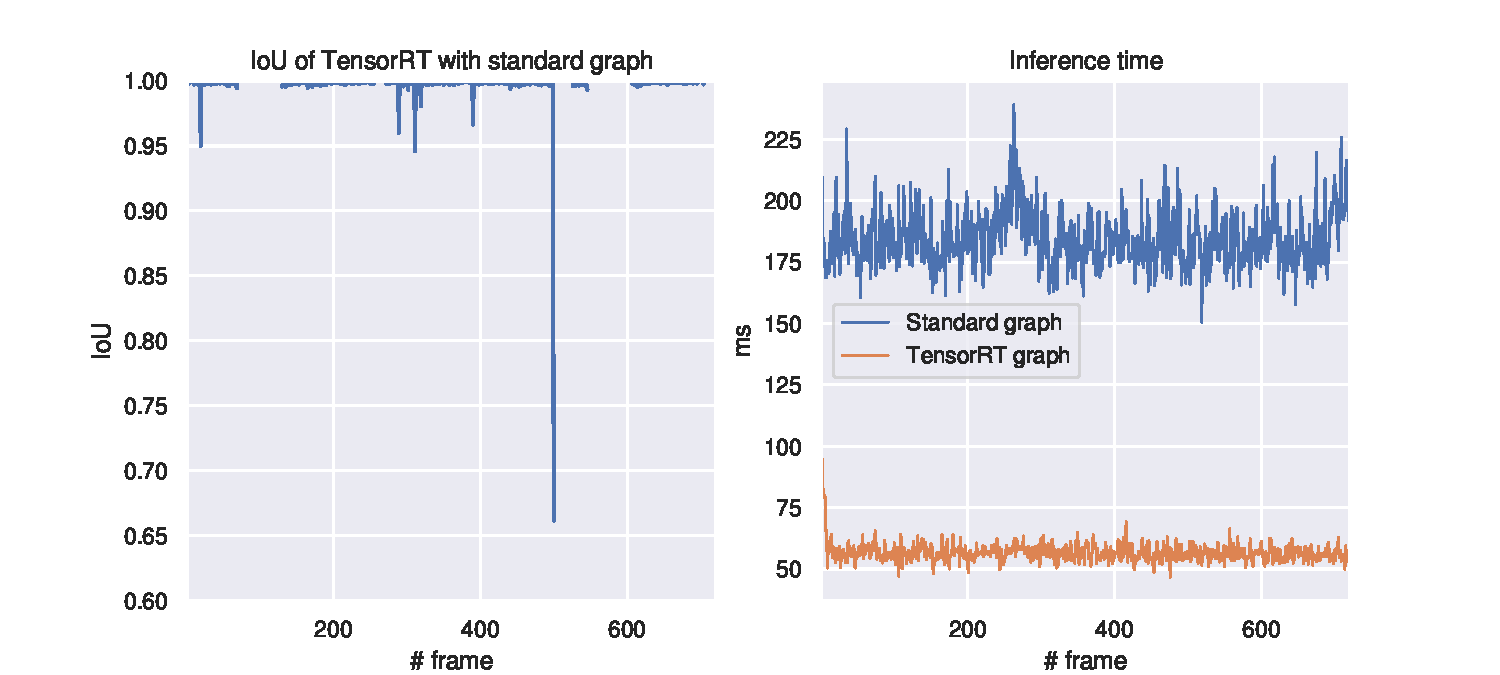
\includegraphics[width=0.85\linewidth]{test3}
	\caption{IoU between the standard graph and the TensorRT graph inferences (left) and inference times for both networks (right). The IoU graph has been rescaled between 0.6 and 1 to have a better visualization of the IoU variability.}
	\label{fig:4_std_vs_trt}
\end{figure}


\begin{table}[h]
	\begin{tabular}{|l|c|c|}
		\hline
		& \textbf{Original graph} & \textbf{TensorRT graph} \\ \hline
		\textbf{Inference time (ms)}           & 184.477 $\pm$  11.827 & 56.769 $\pm$  4.148 \\ \hline
	\end{tabular}
	\caption{Numeric summary (average $\pm$ standard deviation) for the inference time with and without TensorRT.}
	\label{tab:4_test3}
\end{table}


\autoref{fig:4_std_vs_trt} and \autoref{tab:4_test3} illustrate the differences between a standard graph and an optimized one. One of the premises of the optimization process is the reduction of the precision of the parameters in the neural network, which can be reduced from 64-bit values up to 16-bit or even 8-bit (performing an additional quantization process), as it was described on Section \ref{sec:3_design}.\\

The loss of precision is clear as well on \autoref{fig:4_std_vs_trt}, as the IoU of the optimized graph drops at several frames. On the one hand, this loss of precision is small, with some observable exceptions with a loss above 5\% of the original performance. On the other hand, the inference time gap can be observed as well. The difference is more notorious, as the TensorRT optimized model performs the inferences 3 times faster than the original graph (56.769 ms vs. 184.477 ms), as \autoref{tab:4_test3} shows.\\

Given these results, the TensorRT optimizations are a convenient tool to greatly increase the performance of the system, allowing the slower component (the neural pipeline) to experiment an important reduction on the inference time. As a result, the overall performance is greatly improved, receiving reliable neural updates more often.\\

As it was described on Subsection \ref{sec:4_grid_trt}, a set of parameters can be tuned when optimizing a graph with TensorRT, yielding different performances. As \autoref{tab:4_ssd_trt_results} and \autoref{tab:4_yolo_trt_results} show, important reductions on the inference time can be obtained when the rest of parameters (\textit{Maximum Cached Engines} and \textit{Minimum Segment Size}) are tuned as well. However, these parameters only affect the inference time, as the precision loss is only due to the \textit{Precision Mode} parameter, which has been already analyzed.\\

The resulting models can be loaded in the program, instead of the original TensorFlow graphs, and offer an overall higher performance, as it has been demonstrated.






\section{Motion tracker experiments}

\label{sec:4_test5}
In Section \ref{sec:3_design}, the Lucas-Kanade tracker was described. This tracker aims to follow the movements of the person between two consecutive inferences from the neural pipeline. As in embedded systems these inferences might take a long time, an interpolation of the detections using optical flow can be crucial for avoiding a loss of the location of the person, especially if a partial occlusion of the person causes that the network does not detect them for a while.\\

This experiment aims to identify the conditions under which a tracker can palliate these drawbacks of the neural detection pipeline, depending on the parameter $k$. This $k$ modulates the number of elapsed frames between two consecutive neural detections, and takes a higher value if the inferences take longer to be computed by the neural pipeline. On the test, a specific test sequence was recorded and labeled, using a hanging blanket with the purpose of partially occlude the person, making the network to lose the detections. Several frames of the sequence can be visualized on \autoref{fig:3_test5_frames}.\\


\begin{figure}[h]
	\centering
	\begin{subfigure}[b]{0.3\linewidth}
		\centering
		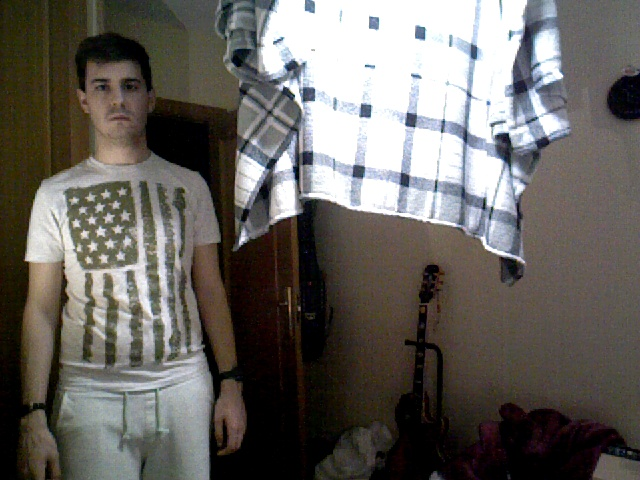
\includegraphics[width=0.95\linewidth]{test5_1}
		\caption{Frame 285.}
	\end{subfigure}
	\begin{subfigure}[b]{0.3\linewidth}
		\centering
		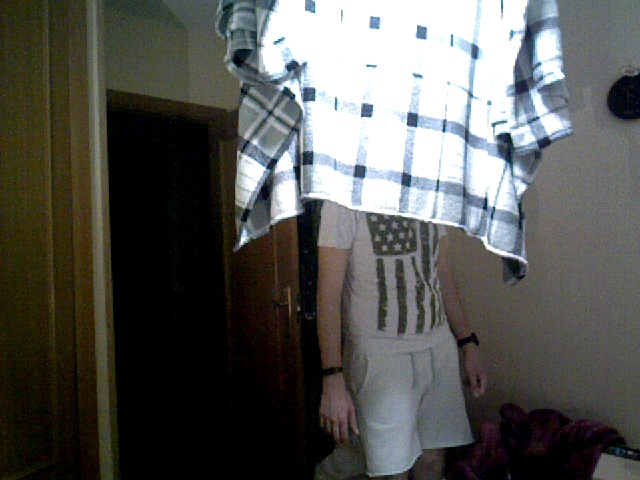
\includegraphics[width=0.95\linewidth]{test5_2}
		\caption{Frame 788.}
	\end{subfigure}
	\begin{subfigure}[b]{0.3\linewidth}
		\centering
		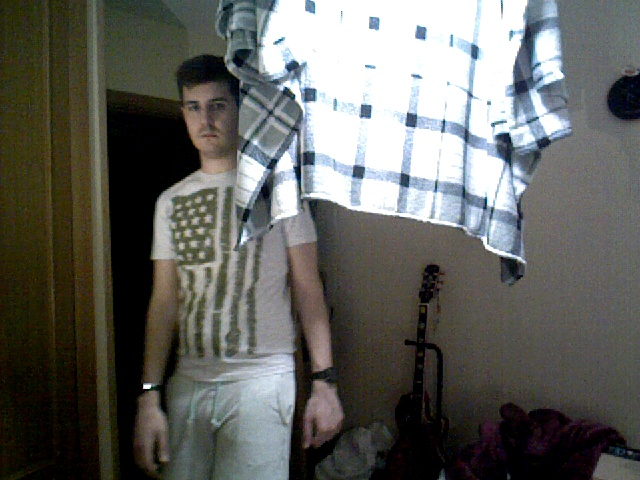
\includegraphics[width=0.95\linewidth]{test5_3}
		\caption{Frame 864.}
	\end{subfigure}
	\caption{3 frames from the test video sequence.}
	\label{fig:3_test5_frames}
\end{figure}



A correctly tuned tracker keeps the detection active and updates the bounding box for a number of frames (determined by the \textit{patience} parameter, as described in Section \ref{sec:3_design}). The video sequence was evaluated using $k=10$ and $k=20$, checking the influence of the tracker in the IoU with the ground truth labels of the sequence. The result for both values of $k$ can be observed on \autoref{fig:3_test5}, where the lapse corresponding to the person occlusion has been emphasized.

\begin{figure}[h]
	\centering
	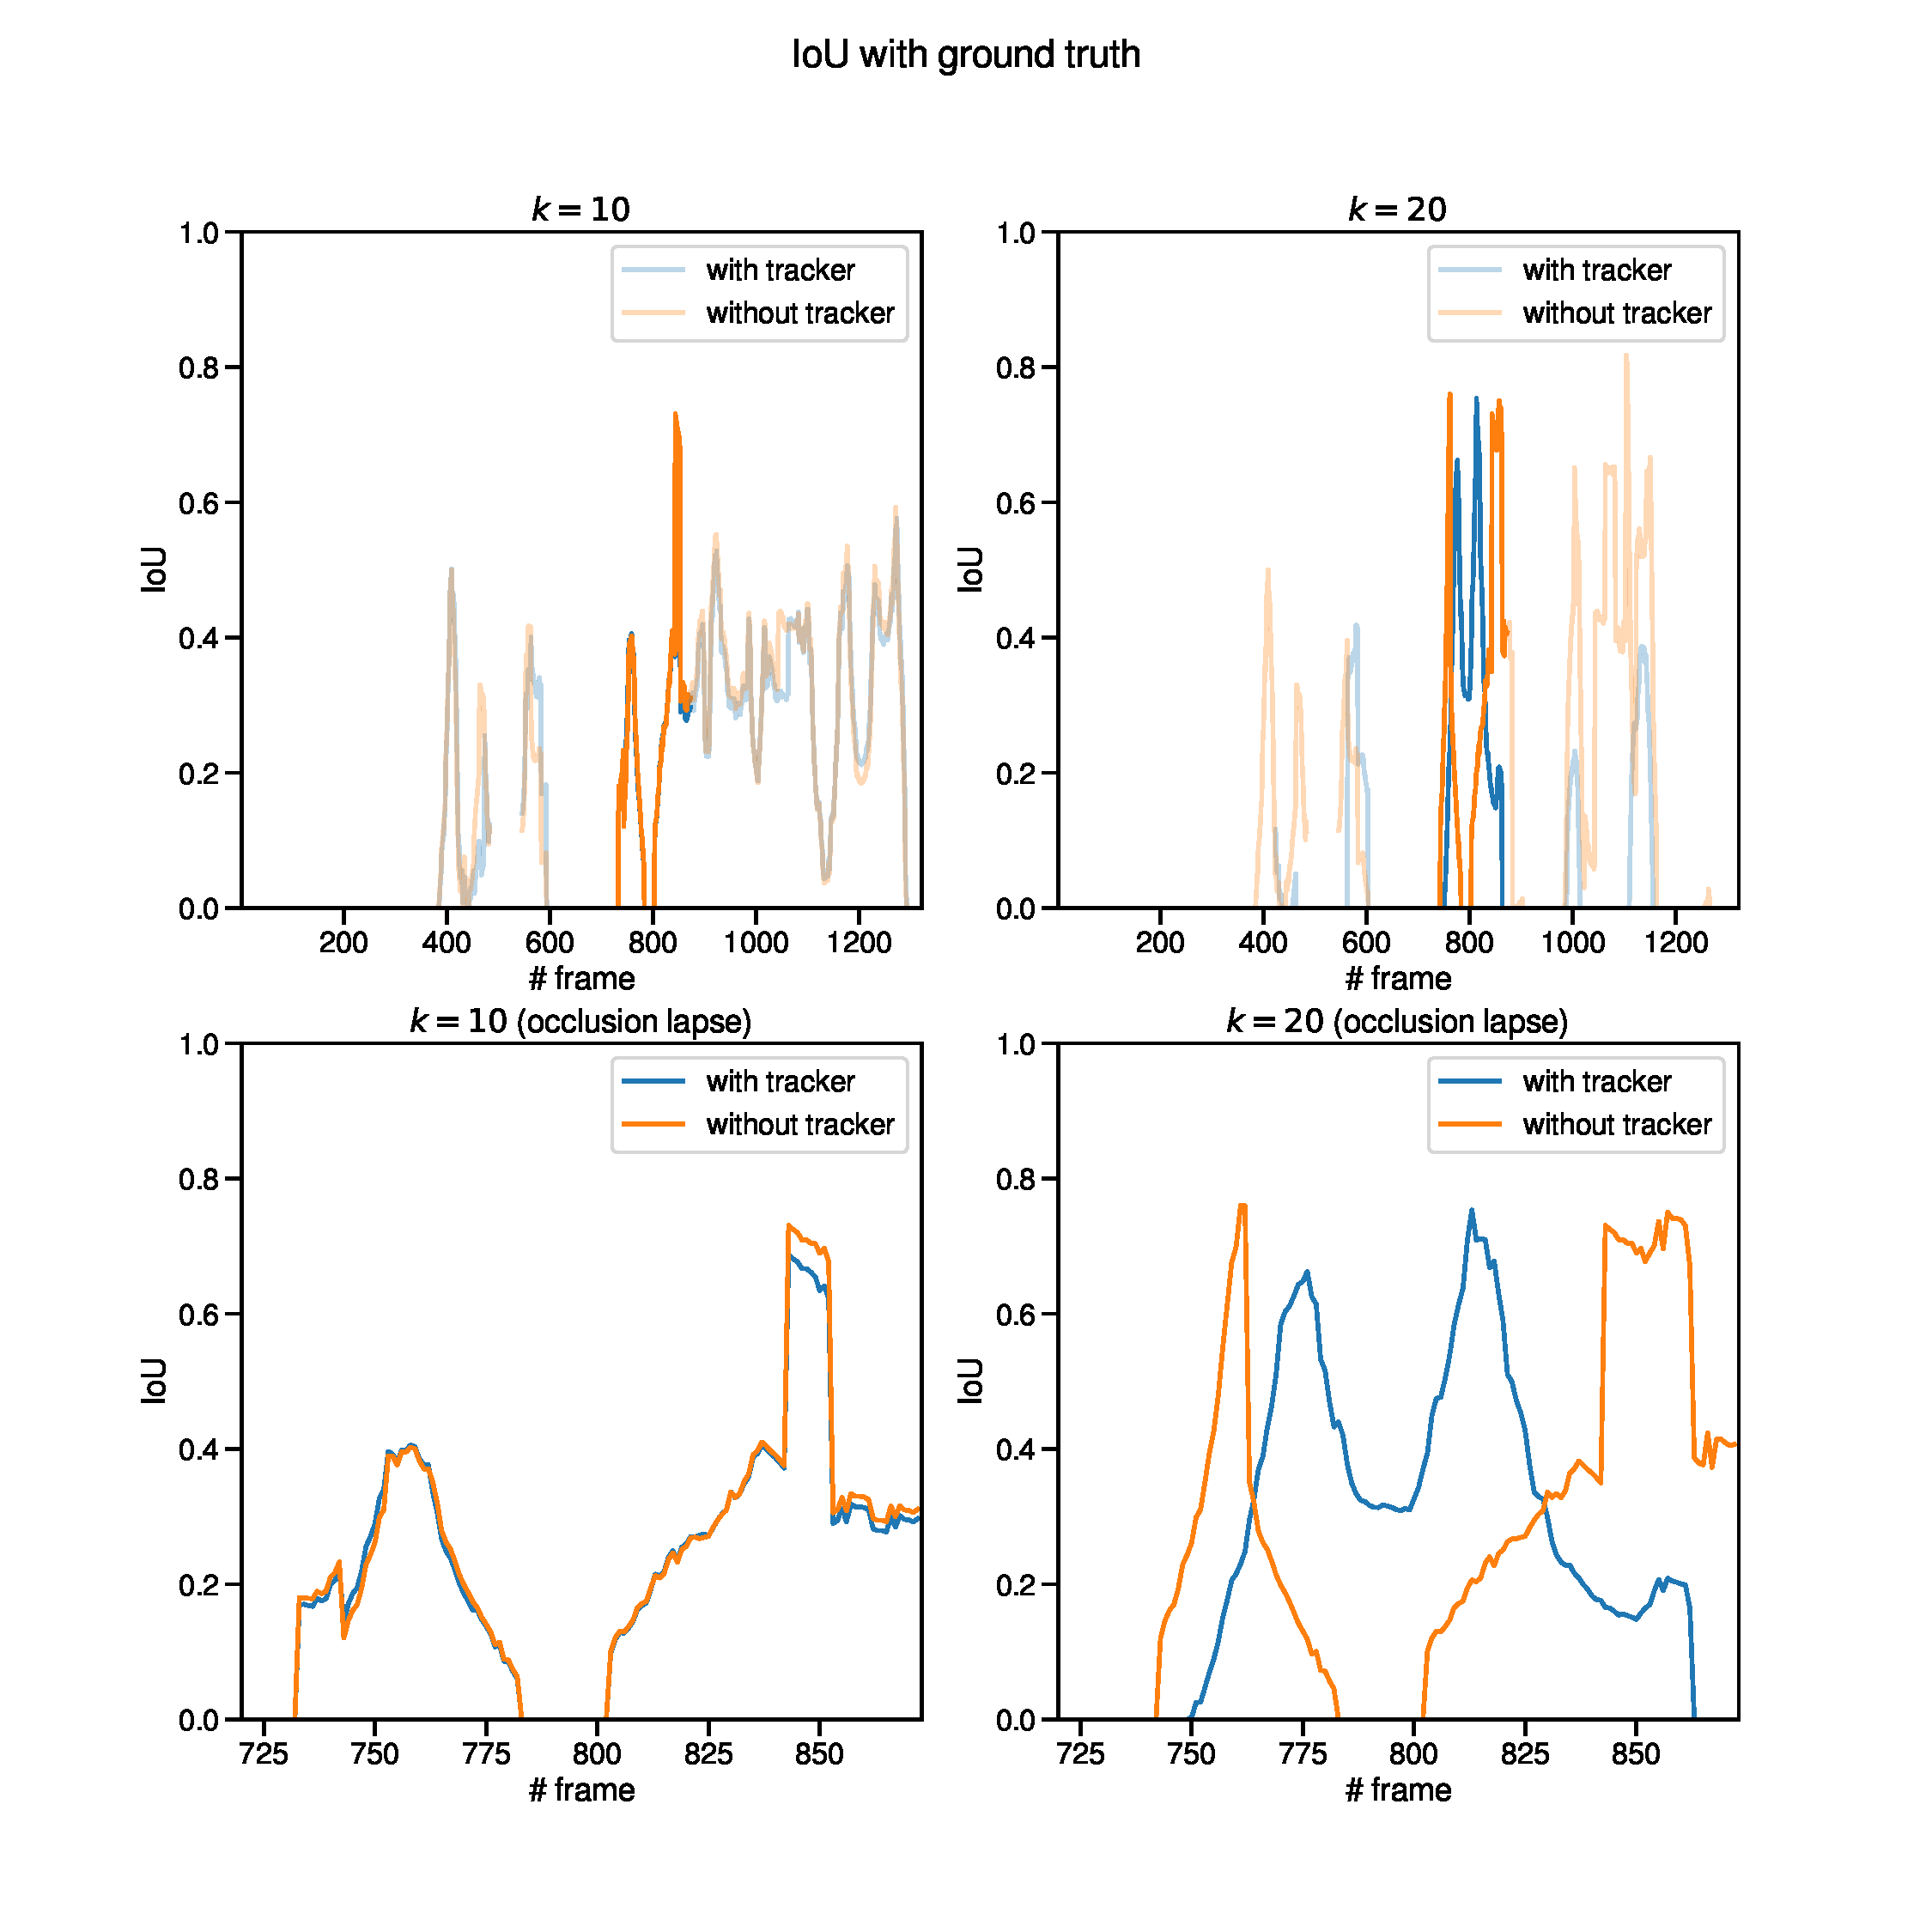
\includegraphics[width=0.85\linewidth]{test5}
	\caption{Results of the motion tracker test, for $k=10$ (left) and $k=20$ (right). The lapse corresponding to the person occlusion has been emphasized and zoomed in in the bottom graphs.}
	\label{fig:3_test5}
\end{figure}


The results on \autoref{fig:3_test5} show the IoU score between the persons and the ground truth labels on the test sequence. Regardless of the value of $k$ (the number of frames elapsed between neural detections), a similar performance can be expected under standard conditions (the faded portion of the graph). However, the emphasized region corresponds to an occlusion behind a hanging blanket (\autoref{fig:3_test5_frames}), and it is zoomed-in on the bottom plots. On this lapse, a better performance is perceptible, especially when the inference time of the neural pipeline is higher ($k=20$). The hanging blanket occludes the person, causing the neural network to stop detecting them. However, as the tracker retains the detection for several updates because of the patience parameter, the person is not lost until several frames later. Additionally, the Lucas-Kanade algorithm allows to determine the displacement of the person even when it is not being detected by the neural pipeline. This explains the higher IoU when the tracker is active due to the bounding box shifting computed using Lucas-Kanade, confirming the improvement in the performance when using the tracker. Outside this region (top plots), some regions can be detected, such as the ending lapse of the sequence  for $k=20$. This is probably due to non-optimal values for the parameters of the tracker, which do not correctly shift the bounding box towards the true direction of movement of the person. A proper in-depth tuning of the parameters can potentially fix this lower performance for situations similar to that lapse.\\



Additionally, while the neural pipeline runs on the GPU of the board, the Lucas-Kanade tracker, whose calculations are much lighter, runs on the CPU. This separation allows to combine both systems asynchronously without affecting the overall load of the system.



\section{Global system experiments}
\label{sec:4_test_full}
Finally, a visual assessment can be derived from a sample of the fully functional system\footnote{\label{footnote:video_url}\url{https://www.youtube.com/watch?v=WZ0riKMwJWA}}. \autoref{fig:3_testfull_frames} shows the behavior of the robot, expected to follow the person properly. The top region of the images shows several screen captures of the program output, with the RGB and depth images (left), and the movement commands and tracked persons (right). The bottom region of the plots show the scene recorded from a mobile phone, allowing to observe the performance externally.\\

\begin{figure}[h]
	\centering
	\begin{subfigure}[t]{0.32\linewidth}
		\centering
		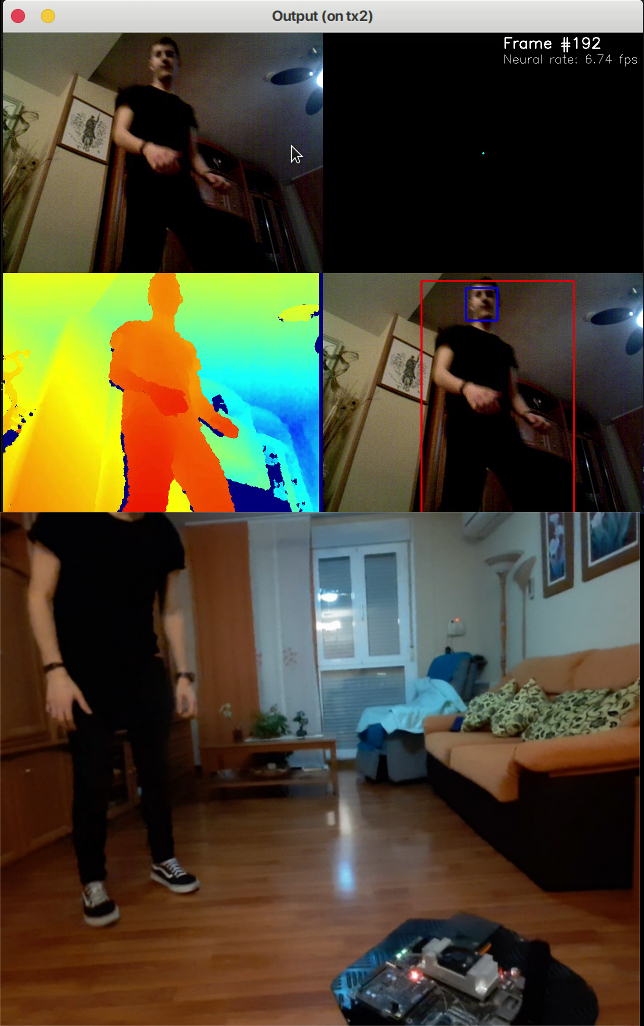
\includegraphics[width=\linewidth]{testfull_1}
		\caption{Person detection.}
	\end{subfigure}
	\begin{subfigure}[t]{0.32\linewidth}
		\centering
		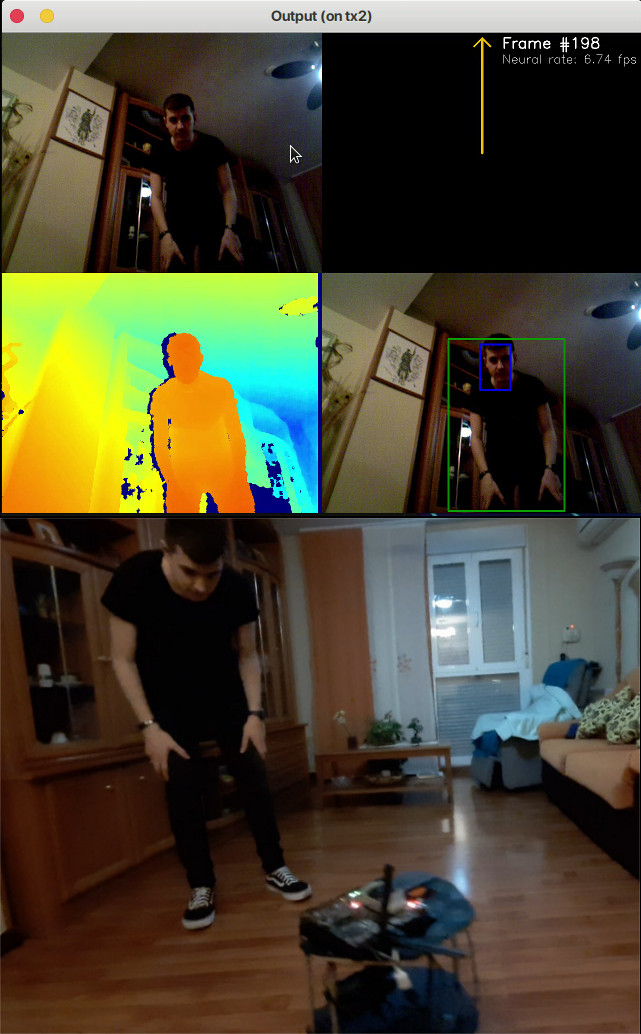
\includegraphics[width=\linewidth]{testfull_2}
		\caption{Person recognition and following.}
	\end{subfigure}
	\begin{subfigure}[t]{0.32\linewidth}
		\centering
		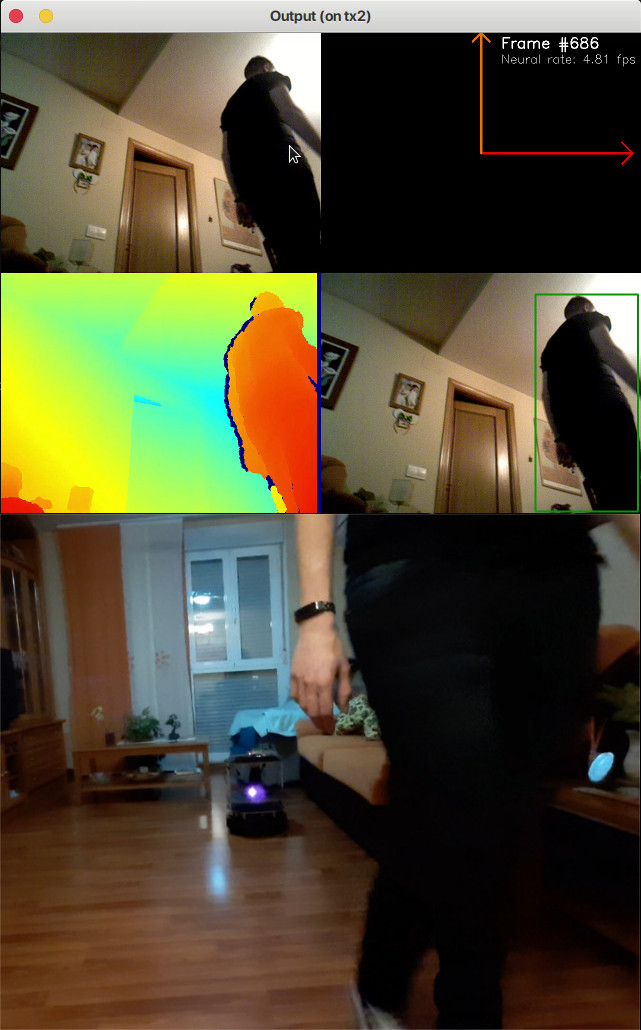
\includegraphics[width=\linewidth]{testfull_3}
		\caption{Following without face feedback.}
	\end{subfigure}
	\caption{3 frames from the full test (available on YouTube, URL on the previous footnote).}
	\label{fig:3_testfull_frames}
\end{figure}



This video presents a sequence of the robot following the typical use case: the reference person enters into the field of view of the robot, showing their face to the camera. After some consecutive frames detecting the person, it is identified using the detected face. When its projection is close enough to the reference one, the robot starts following the person. For each frame, the linear and angular errors are computed, even if the face of the person is not seen anymore, as the system has checked previously that the person has to be followed. If the errors are outside the safe zones, a velocity command is computed and sent to the robot. This routine is executed iteratively until the person gets lost, causing the robot to stop waiting for the person to be seen again.



